\documentclass[10pt]{beamer}
\usetheme[
%%% option passed to the outer theme
%    progressstyle=fixedCircCnt,   % fixedCircCnt, movingCircCnt (moving is deault)
  ]{Feather}
  
% If you want to change the colors of the various elements in the theme, edit and uncomment the following lines

% Change the bar colors:
%\setbeamercolor{Feather}{fg=red!20,bg=red}

% Change the color of the structural elements:
%\setbeamercolor{structure}{fg=red}

% Change the frame title text color:
%\setbeamercolor{frametitle}{fg=blue}

% Change the normal text color background:
%\setbeamercolor{normal text}{fg=black,bg=gray!10}

%-------------------------------------------------------
% INCLUDE PACKAGES
%-------------------------------------------------------

\usepackage[utf8]{inputenc}
\usepackage[english]{babel}
\usepackage[T1]{fontenc}
\usepackage{helvet}

%-------------------------------------------------------
% DEFFINING AND REDEFINING COMMANDS
%-------------------------------------------------------

% colored hyperlinks
\newcommand{\chref}[2]{
  \href{#1}{{\usebeamercolor[bg]{Feather}#2}}
}

%-------------------------------------------------------
% INFORMATION IN THE TITLE PAGE
%-------------------------------------------------------

\title[] % [] is optional - is placed on the bottom of the sidebar on every slide
{ % is placed on the title page
      \textbf{Bezbedno traženje biomarkera korišćenjem hibridne homomorfne enkripcione šeme}
}


\author[Una Stanković]
{      Una Stanković \\
      {\ttfamily una\_stankovic@yahoo.com}
}

\institute[]
{
      Matematički fakultet\\
      Univerzitet u Beogradu\\
  
  %there must be an empty line above this line - otherwise some unwanted space is added between the university and the country (I do not know why;( )
}

\date{\today}

%-------------------------------------------------------
% THE BODY OF THE PRESENTATION
%-------------------------------------------------------

\begin{document}

%-------------------------------------------------------
% THE TITLEPAGE
%-------------------------------------------------------

{\1% % this is the name of the PDF file for the background
\begin{frame}[plain,noframenumbering] % the plain option removes the header from the title page, noframenumbering removes the numbering of this frame only
  \titlepage % call the title page information from above
\end{frame}}


\begin{frame}{Sadržaj}{}
\tableofcontents
\end{frame}

%-------------------------------------------------------
\section{Uvod}
%-------------------------------------------------------
\begin{frame}{Uvod}
%-------------------------------------------------------
\begin{block}{Motivacija}
\begin{itemize}
\item brz razvoj tehnologija sekvenciranja genoma
\item pristup velikim skupovima genoma
\item veliki potencijal u razvoju biomedicinskih istraživanja
\item primene u:
	\begin{itemize}
	\item medicini,
	\item biomedicinskim istraživanjima,
	\item uslugama koje se direktno pružaju korisnicima,...
\end{itemize}	 
\end{itemize}

\end{block}
\end{frame}

\begin{frame}{Uvod}
\begin{figure}[H]
 	\centering
	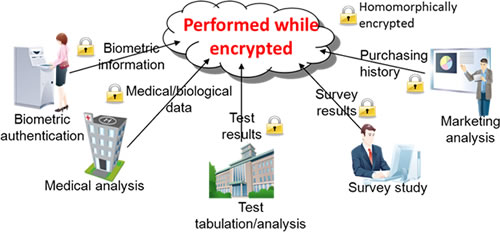
\includegraphics[width=\textwidth,height=\textheight,keepaspectratio]{slika1.jpg}
 	\caption{Idejni prikaz.}
 	\label{fig:primer}
 \end{figure}
\end{frame}

\begin{frame}{Homomorfna enkripcija}
%-------------------------------------------------------
\begin{block}{Osnovna ideja}
	\begin{itemize}
		\item izvodimo operacije nad enkriptovanim tekstom
		\item dobijamo enkriptovani rezultat
		\item dekriptujemo dobijeni rezultat
		\item konačni rezultat je isti kao da smo primenili operacije nad neekriptovanim tekstom
	\end{itemize}
\end{block}
\end{frame}

%-------------------------------------------------------
\section{Postavka problema}
%-------------------------------------------------------
\begin{frame}{Postavka problema}{Zadatak}
%-------------------------------------------------------
\begin{block}{}
	Zadatak je da se na bezbedan način izračuna verovatnoća genetskih
bolesti kroz uparivanje skupa biomarkera sa enkriptovanim genomima koji
se čuvaju u javnom "oblaku"(engl. cloud).
\end{block}
\end{frame}

\begin{frame}
%-------------------------------------------------------
\begin{figure}[H]
 	\centering
	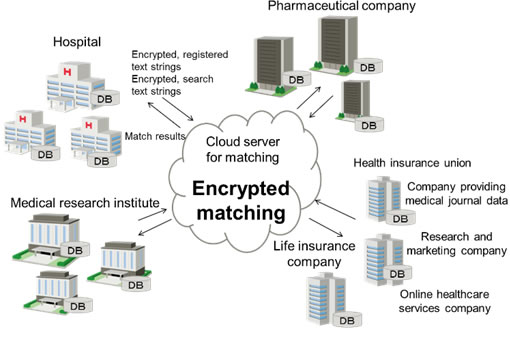
\includegraphics[width=\textwidth,height=\textheight,keepaspectratio]{slika2.jpg}
 	\label{fig:primer}
 \end{figure}
\end{frame}

\section{Postupak}
\begin{frame}{Postupak}
%-------------------------------------------------------
\begin{block}{Uslovi}
	\begin{enumerate}
		\item proces uparivanja mora biti izvršen korišćenjem homomorfne enkripcije
		\item serveru se ne smeju otkriti informacije o bazi ili upitu
	\end{enumerate}			
\end{block}
\begin{figure}[H]
 	\centering
	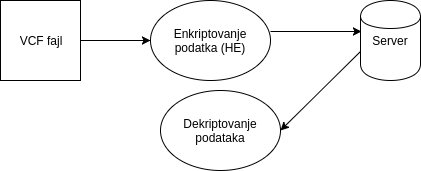
\includegraphics[width=\textwidth,height=\textheight,keepaspectratio]{slika3.png}
 	\label{fig:primer}
 \end{figure}
\end{frame}



%-------------------------------------------------------
\section{Pretraga i izvlačenje podataka iz baze}
\begin{frame}{Pretraga i izvlačenje podataka iz baze}{Osnovna ideja}
%-------------------------------------------------------
\begin{block}{}
\begin{itemize}
\item Baza je skup n torki
\item Svaka torka se sastoji iz ($d_i$, $\alpha_i$)
\item $d_i$ pripadaju nekom domenu, $\alpha_i$ su odgovarajuće vrednosti atributa u prostoru običnog teksta 
\item Pojednostavljeni upit za pretragu : \textit{odaberi $\alpha_i$ ako postoji indeks \textbf{i} takav da je $d_i$ = d, inače nula.}
%\item Server ne sme da nauči ništa iz enkriptovanog upita
%\item Klijent ne sme da dobije ništa osim krajnjeg rezultata
\end{itemize}
\end{block}

\end{frame}

\subsection{Metod za bezbednu pretragu i izvlačenje podataka}
\begin{frame}{Metod za bezbednu pretragu i izvlačenje podataka}
\begin{block}{Metod za enkodiranje baze}
	\begin{itemize}
		\item pogodan za efikasno izračunavanje jednakosti i izvlačenje podataka
		\item $$DB(X) = \sum_{i} \alpha_i X^{d_i} \in \mathbb{Z}$$
		\item Postupak 
		\begin{enumerate}
			\item korisnik enkriptuje polinom sa javnim ključem
			\item šifrovani tekst se čuva na serveru
			\item u fazi ispitivanja upita sa nazivom d, korisnik enkriptuje $X^{-d}$ sa simetričnom enkripcijom
			\item šifrovani tekst šalje ka serveru.
		\end{enumerate}
	\end{itemize}
\end{block}
\end{frame}
     

%-------------------------------------------------------
\subsection{Bezbedna pretraga biomarkera}
\begin{frame}{Bezbedna pretraga biomarkera}{Enkodiranje informacija o genomu}
%-------------------------------------------------------
\begin{block}{}
\begin{itemize}
\item VCF fajl sadrži informacije o genotipu: ($ch_i$,$pos_i$, SNP$s_i$) tj. broj hromozoma, pozicije i sekvence SNP alela (koji moraju biti A, T, G ili C)
\item Upit korisnika je, isto, triplet ovakvog oblika 
\item Cilj je da odredimo postoji li ili ne prisustvo odgovarajućeg biomarkera u fajlu iz baze
\item $n_SNP$ je maksimalni broj alela, koje kodiramo kao: $$A \rightarrow 00, T \rightarrow 01, G \rightarrow 10, C \rightarrow 11$$
\item Stavljamo bit 1 na početak stringa sa leve strane da označimo početnu poziciju
\item Popunjavamo string dužine $\textit{l}_{SNP}$ = 2$n_{SNP}$ + 1 i konvertujemo dobijeno u ceo broj, označen sa $\alpha_i$
\end{itemize}
\end{block}
\end{frame}

%\subsection{Bezbedna pretraga biomarkera}
%\begin{frame}{Bezbedna pretraga biomarkera}{Enkriptovanje informacija o genomu}
%-------------------------------------------------------
%\begin{block}{}
%\begin{itemize}
%\item Baza je skup n torki
%\item Svaka torka se sastoji iz ($d_i$, $\alpha_i$)
%\item $d_i$ pripadaju nekom domenu, $\alpha_i$ su odgovarajuće vrednosti atributa u prostoru običnog teksta 
%\item Pojednostavljeni upit za pretragu : \textit{odaberi $\alpha_i$ ako postoji indeks \textbf{i} takav da je $d_i$ = d, inače nula.}
%\item Server ne sme da nauči ništa iz enkriptovanog upita
%\item Klijent ne sme da dobije ništa osim krajnjeg rezultata
%\end{itemize}
%\end{block}
  
%\end{frame}

%-------------------------------------------------------
\section{Literatura}
\begin{frame}{Literatura}
%-------------------------------------------------------
\begin{itemize}
\item Jung Hee Cheon, Miran Kim, Yongsoo Song, "Secure Searching of Biomarkers Using Hybrid Homomorphic Encryption Scheme"\\ http://eprint.iacr.org/2017/294.pdf
\end{itemize}

\end{frame}


{\1
\begin{frame}[plain,noframenumbering]
  \finalpage{Hvala na pažnji!}
\end{frame}}

\end{document}